\documentclass[tikz, border=10pt]{standalone}
\usepackage{tikz}
\usetikzlibrary{positioning, arrows.meta, shapes, backgrounds, fit, calc}

\begin{document}

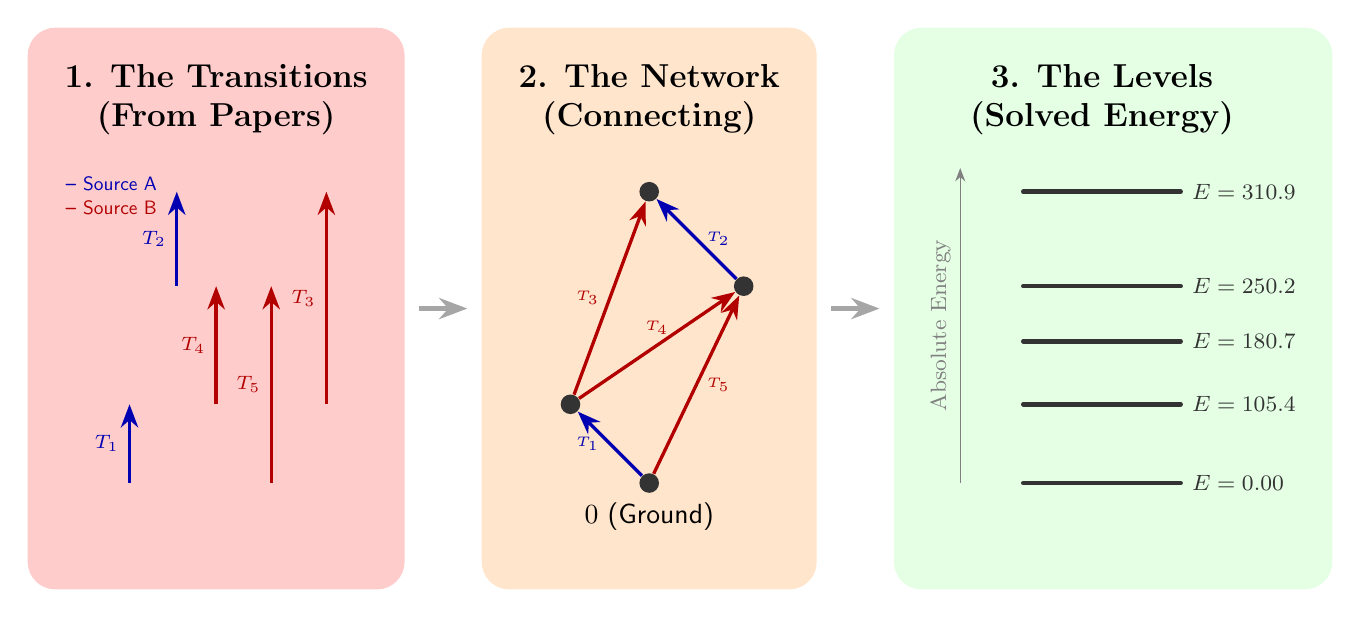
\begin{tikzpicture}[
    % Global Styles
    font=\sffamily,
    >=Stealth,
    node distance=1cm,
    % Style for energy dots and lines
    level_dot/.style={circle, fill=black!80, inner sep=2.5pt},
    level_line/.style={ultra thick, black!80, line cap=round},
    % --- STYLES FOR SOURCES ---
    srcA/.style={->, very thick, color=blue!70!black},
    srcB/.style={->, very thick, color=red!70!black},
    % Style for the colored panels
    panel_bg/.style={rounded corners=10pt, inner sep=10pt, draw=none},
    % Style for headings
    heading/.style={font=\bfseries\large, align=center, anchor=south}
]

%% --- PANEL 1: INPUT (RAW DATA) ---
\begin{scope}[local bounding box=p1]
    % INVISIBLE STRUT for height alignment
    \path (0,-1.5) -- (0,4.5); 

    % Heading
    \node[heading] at (1.5, 3.8) {1. The Transitions\\(From Papers)};
    
    % Legend
    \node[right, scale=0.7, text=blue!70!black] at (-0.5, 3.3) {\textbf{--} Source A};
    \node[right, scale=0.7, text=red!70!black] at (-0.5, 3.0) {\textbf{--} Source B};

    % TRANSFORMED TRANSITIONS: 
    % Vertical lines floating at the exact heights of the nodes in Panel 2
    
    % --- Source A (Blue) ---
    % T1: Connects Ground (-0.5) to A (0.5)
    \draw[srcA] (0.4, -0.5) -- (0.4, 0.5) node[midway, left, font=\scriptsize] {$T_1$};
    
    % T2: Connects B (2.0) to C (3.2) -> Floats high up
    \draw[srcA] (1.0, 2.0) -- (1.0, 3.2) node[midway, left, font=\scriptsize] {$T_2$};
    
    % --- Source B (Red) ---
    % T4: Connects A (0.5) to B (2.0) -> Floats in middle
    \draw[srcB] (1.5, 0.5) -- (1.5, 2.0) node[midway, left, font=\scriptsize] {$T_4$};
    
    % T5: Connects Ground (-0.5) to B (2.0) -> Long arrow from bottom
    \draw[srcB] (2.2, -0.5) -- (2.2, 2.0) node[midway, left, font=\scriptsize] {$T_5$};
    
    % T3: Connects A (0.5) to C (3.2) -> Long arrow from middle
    \draw[srcB] (2.9, 0.5) -- (2.9, 3.2) node[midway, left, font=\scriptsize] {$T_3$};

\end{scope}

%% --- PANEL 2: NETWORK (GRAPH) ---
\begin{scope}[xshift=6.0cm, local bounding box=p2]
    % INVISIBLE STRUT
    \path (0,-1.5) -- (0,4.5);

    % Heading
    \node[heading] at (1, 3.8) {2. The Network\\(Connecting)};

    % Nodes (Energy Levels)
    % G = Ground (y = -0.5)
    \node[level_dot, label=below:{$0$ (Ground)}] (G) at (1, -0.5) {};
    % A = Low (y = 0.5)
    \node[level_dot] (A) at (0, 0.5) {};
    % B = High (y = 2.0)
    \node[level_dot] (B) at (2.2, 2.0) {};
    % C = Highest (y = 3.2)
    \node[level_dot] (C) at (1, 3.2) {};
    
    % Connections 
    % Source A
    \draw[srcA] (G) -- (A) node[midway, left, font=\tiny] {$T_1$};
    \draw[srcA] (B) -- (C) node[midway, right, font=\tiny] {$T_2$};
    
    % Source B
    \draw[srcB] (G) -- (B) node[midway, right, font=\tiny] {$T_5$}; 
    \draw[srcB] (A) -- (C) node[midway, left, font=\tiny] {$T_3$};
    \draw[srcB] (A) -- (B) node[midway, above, font=\tiny] {$T_4$}; 
\end{scope}

%% --- PANEL 3: OUTPUT (LEVELS) ---
\begin{scope}[xshift=11.75cm, local bounding box=p3]
    % INVISIBLE STRUT
    \path (0,-1.5) -- (0,4.5);

    % Heading
    \node[heading] at (1, 3.8) {3. The Levels\\(Solved Energy)};

    % Ladder (5 Levels)
    \draw[level_line] (0,-0.5) -- (2,-0.5) node[right, font=\footnotesize] {$E=0.00$};
    \draw[level_line] (0,0.5) -- (2,0.5) node[right, font=\footnotesize] {$E=105.4$};
    \draw[level_line] (0,1.3) -- (2,1.3) node[right, font=\footnotesize] {$E=180.7$};
    \draw[level_line] (0,2.0) -- (2,2.0) node[right, font=\footnotesize] {$E=250.2$};
    \draw[level_line] (0,3.2) -- (2,3.2) node[right, font=\footnotesize] {$E=310.9$};
    
    % Axis Arrow
    \draw[->, thin, gray] (-0.8, -0.5) -- (-0.8, 3.5);
    \node[gray, rotate=90, font=\footnotesize, anchor=south] at (-0.8, 1.5) {Absolute Energy};
\end{scope}

%% --- BACKGROUND LAYERS ---
\begin{scope}[on background layer]
    % Panel 1: More Red
    \node[panel_bg, fill=red!20, fit=(p1)] (bg1) {};
    % Panel 2: More Orange/Yellow
    \node[panel_bg, fill=orange!20, fit=(p2)] (bg2) {};
    % Panel 3: Green
    \node[panel_bg, fill=green!10, fit=(p3)] (bg3) {};
\end{scope}

%% --- FLOW ARROWS BETWEEN PANELS ---
\draw[->, ultra thick, gray!70, shorten >= 5pt, shorten <= 5pt] (bg1.east) -- (bg2.west);
\draw[->, ultra thick, gray!70, shorten >= 5pt, shorten <= 5pt] (bg2.east) -- (bg3.west);

\end{tikzpicture}
\end{document}